\documentclass{article} % For LaTeX2e
\usepackage{iclr2027_conference,times}

% Optional math commands from https://github.com/goodfeli/dlbook_notation.
%%%%% NEW MATH DEFINITIONS %%%%%

\usepackage{amsmath,amsfonts,bm}

% Mark sections of captions for referring to divisions of figures
\newcommand{\figleft}{{\em (Left)}}
\newcommand{\figcenter}{{\em (Center)}}
\newcommand{\figright}{{\em (Right)}}
\newcommand{\figtop}{{\em (Top)}}
\newcommand{\figbottom}{{\em (Bottom)}}
\newcommand{\captiona}{{\em (a)}}
\newcommand{\captionb}{{\em (b)}}
\newcommand{\captionc}{{\em (c)}}
\newcommand{\captiond}{{\em (d)}}

% Highlight a newly defined term
\newcommand{\newterm}[1]{{\bf #1}}


% Figure reference, lower-case.
\def\figref#1{figure~\ref{#1}}
% Figure reference, capital. For start of sentence
\def\Figref#1{Figure~\ref{#1}}
\def\twofigref#1#2{figures \ref{#1} and \ref{#2}}
\def\quadfigref#1#2#3#4{figures \ref{#1}, \ref{#2}, \ref{#3} and \ref{#4}}
% Section reference, lower-case.
\def\secref#1{section~\ref{#1}}
% Section reference, capital.
\def\Secref#1{Section~\ref{#1}}
% Reference to two sections.
\def\twosecrefs#1#2{sections \ref{#1} and \ref{#2}}
% Reference to three sections.
\def\secrefs#1#2#3{sections \ref{#1}, \ref{#2} and \ref{#3}}
% Reference to an equation, lower-case.
\def\eqref#1{equation~\ref{#1}}
% Reference to an equation, upper case
\def\Eqref#1{Equation~\ref{#1}}
% A raw reference to an equation---avoid using if possible
\def\plaineqref#1{\ref{#1}}
% Reference to a chapter, lower-case.
\def\chapref#1{chapter~\ref{#1}}
% Reference to an equation, upper case.
\def\Chapref#1{Chapter~\ref{#1}}
% Reference to a range of chapters
\def\rangechapref#1#2{chapters\ref{#1}--\ref{#2}}
% Reference to an algorithm, lower-case.
\def\algref#1{algorithm~\ref{#1}}
% Reference to an algorithm, upper case.
\def\Algref#1{Algorithm~\ref{#1}}
\def\twoalgref#1#2{algorithms \ref{#1} and \ref{#2}}
\def\Twoalgref#1#2{Algorithms \ref{#1} and \ref{#2}}
% Reference to a part, lower case
\def\partref#1{part~\ref{#1}}
% Reference to a part, upper case
\def\Partref#1{Part~\ref{#1}}
\def\twopartref#1#2{parts \ref{#1} and \ref{#2}}

\def\ceil#1{\lceil #1 \rceil}
\def\floor#1{\lfloor #1 \rfloor}
\def\1{\bm{1}}
\newcommand{\train}{\mathcal{D}}
\newcommand{\valid}{\mathcal{D_{\mathrm{valid}}}}
\newcommand{\test}{\mathcal{D_{\mathrm{test}}}}

\def\eps{{\epsilon}}


% Random variables
\def\reta{{\textnormal{$\eta$}}}
\def\ra{{\textnormal{a}}}
\def\rb{{\textnormal{b}}}
\def\rc{{\textnormal{c}}}
\def\rd{{\textnormal{d}}}
\def\re{{\textnormal{e}}}
\def\rf{{\textnormal{f}}}
\def\rg{{\textnormal{g}}}
\def\rh{{\textnormal{h}}}
\def\ri{{\textnormal{i}}}
\def\rj{{\textnormal{j}}}
\def\rk{{\textnormal{k}}}
\def\rl{{\textnormal{l}}}
% rm is already a command, just don't name any random variables m
\def\rn{{\textnormal{n}}}
\def\ro{{\textnormal{o}}}
\def\rp{{\textnormal{p}}}
\def\rq{{\textnormal{q}}}
\def\rr{{\textnormal{r}}}
\def\rs{{\textnormal{s}}}
\def\rt{{\textnormal{t}}}
\def\ru{{\textnormal{u}}}
\def\rv{{\textnormal{v}}}
\def\rw{{\textnormal{w}}}
\def\rx{{\textnormal{x}}}
\def\ry{{\textnormal{y}}}
\def\rz{{\textnormal{z}}}

% Random vectors
\def\rvepsilon{{\mathbf{\epsilon}}}
\def\rvtheta{{\mathbf{\theta}}}
\def\rva{{\mathbf{a}}}
\def\rvb{{\mathbf{b}}}
\def\rvc{{\mathbf{c}}}
\def\rvd{{\mathbf{d}}}
\def\rve{{\mathbf{e}}}
\def\rvf{{\mathbf{f}}}
\def\rvg{{\mathbf{g}}}
\def\rvh{{\mathbf{h}}}
\def\rvu{{\mathbf{i}}}
\def\rvj{{\mathbf{j}}}
\def\rvk{{\mathbf{k}}}
\def\rvl{{\mathbf{l}}}
\def\rvm{{\mathbf{m}}}
\def\rvn{{\mathbf{n}}}
\def\rvo{{\mathbf{o}}}
\def\rvp{{\mathbf{p}}}
\def\rvq{{\mathbf{q}}}
\def\rvr{{\mathbf{r}}}
\def\rvs{{\mathbf{s}}}
\def\rvt{{\mathbf{t}}}
\def\rvu{{\mathbf{u}}}
\def\rvv{{\mathbf{v}}}
\def\rvw{{\mathbf{w}}}
\def\rvx{{\mathbf{x}}}
\def\rvy{{\mathbf{y}}}
\def\rvz{{\mathbf{z}}}

% Elements of random vectors
\def\erva{{\textnormal{a}}}
\def\ervb{{\textnormal{b}}}
\def\ervc{{\textnormal{c}}}
\def\ervd{{\textnormal{d}}}
\def\erve{{\textnormal{e}}}
\def\ervf{{\textnormal{f}}}
\def\ervg{{\textnormal{g}}}
\def\ervh{{\textnormal{h}}}
\def\ervi{{\textnormal{i}}}
\def\ervj{{\textnormal{j}}}
\def\ervk{{\textnormal{k}}}
\def\ervl{{\textnormal{l}}}
\def\ervm{{\textnormal{m}}}
\def\ervn{{\textnormal{n}}}
\def\ervo{{\textnormal{o}}}
\def\ervp{{\textnormal{p}}}
\def\ervq{{\textnormal{q}}}
\def\ervr{{\textnormal{r}}}
\def\ervs{{\textnormal{s}}}
\def\ervt{{\textnormal{t}}}
\def\ervu{{\textnormal{u}}}
\def\ervv{{\textnormal{v}}}
\def\ervw{{\textnormal{w}}}
\def\ervx{{\textnormal{x}}}
\def\ervy{{\textnormal{y}}}
\def\ervz{{\textnormal{z}}}

% Random matrices
\def\rmA{{\mathbf{A}}}
\def\rmB{{\mathbf{B}}}
\def\rmC{{\mathbf{C}}}
\def\rmD{{\mathbf{D}}}
\def\rmE{{\mathbf{E}}}
\def\rmF{{\mathbf{F}}}
\def\rmG{{\mathbf{G}}}
\def\rmH{{\mathbf{H}}}
\def\rmI{{\mathbf{I}}}
\def\rmJ{{\mathbf{J}}}
\def\rmK{{\mathbf{K}}}
\def\rmL{{\mathbf{L}}}
\def\rmM{{\mathbf{M}}}
\def\rmN{{\mathbf{N}}}
\def\rmO{{\mathbf{O}}}
\def\rmP{{\mathbf{P}}}
\def\rmQ{{\mathbf{Q}}}
\def\rmR{{\mathbf{R}}}
\def\rmS{{\mathbf{S}}}
\def\rmT{{\mathbf{T}}}
\def\rmU{{\mathbf{U}}}
\def\rmV{{\mathbf{V}}}
\def\rmW{{\mathbf{W}}}
\def\rmX{{\mathbf{X}}}
\def\rmY{{\mathbf{Y}}}
\def\rmZ{{\mathbf{Z}}}

% Elements of random matrices
\def\ermA{{\textnormal{A}}}
\def\ermB{{\textnormal{B}}}
\def\ermC{{\textnormal{C}}}
\def\ermD{{\textnormal{D}}}
\def\ermE{{\textnormal{E}}}
\def\ermF{{\textnormal{F}}}
\def\ermG{{\textnormal{G}}}
\def\ermH{{\textnormal{H}}}
\def\ermI{{\textnormal{I}}}
\def\ermJ{{\textnormal{J}}}
\def\ermK{{\textnormal{K}}}
\def\ermL{{\textnormal{L}}}
\def\ermM{{\textnormal{M}}}
\def\ermN{{\textnormal{N}}}
\def\ermO{{\textnormal{O}}}
\def\ermP{{\textnormal{P}}}
\def\ermQ{{\textnormal{Q}}}
\def\ermR{{\textnormal{R}}}
\def\ermS{{\textnormal{S}}}
\def\ermT{{\textnormal{T}}}
\def\ermU{{\textnormal{U}}}
\def\ermV{{\textnormal{V}}}
\def\ermW{{\textnormal{W}}}
\def\ermX{{\textnormal{X}}}
\def\ermY{{\textnormal{Y}}}
\def\ermZ{{\textnormal{Z}}}

% Vectors
\def\vzero{{\bm{0}}}
\def\vone{{\bm{1}}}
\def\vmu{{\bm{\mu}}}
\def\vtheta{{\bm{\theta}}}
\def\va{{\bm{a}}}
\def\vb{{\bm{b}}}
\def\vc{{\bm{c}}}
\def\vd{{\bm{d}}}
\def\ve{{\bm{e}}}
\def\vf{{\bm{f}}}
\def\vg{{\bm{g}}}
\def\vh{{\bm{h}}}
\def\vi{{\bm{i}}}
\def\vj{{\bm{j}}}
\def\vk{{\bm{k}}}
\def\vl{{\bm{l}}}
\def\vm{{\bm{m}}}
\def\vn{{\bm{n}}}
\def\vo{{\bm{o}}}
\def\vp{{\bm{p}}}
\def\vq{{\bm{q}}}
\def\vr{{\bm{r}}}
\def\vs{{\bm{s}}}
\def\vt{{\bm{t}}}
\def\vu{{\bm{u}}}
\def\vv{{\bm{v}}}
\def\vw{{\bm{w}}}
\def\vx{{\bm{x}}}
\def\vy{{\bm{y}}}
\def\vz{{\bm{z}}}

% Elements of vectors
\def\evalpha{{\alpha}}
\def\evbeta{{\beta}}
\def\evepsilon{{\epsilon}}
\def\evlambda{{\lambda}}
\def\evomega{{\omega}}
\def\evmu{{\mu}}
\def\evpsi{{\psi}}
\def\evsigma{{\sigma}}
\def\evtheta{{\theta}}
\def\eva{{a}}
\def\evb{{b}}
\def\evc{{c}}
\def\evd{{d}}
\def\eve{{e}}
\def\evf{{f}}
\def\evg{{g}}
\def\evh{{h}}
\def\evi{{i}}
\def\evj{{j}}
\def\evk{{k}}
\def\evl{{l}}
\def\evm{{m}}
\def\evn{{n}}
\def\evo{{o}}
\def\evp{{p}}
\def\evq{{q}}
\def\evr{{r}}
\def\evs{{s}}
\def\evt{{t}}
\def\evu{{u}}
\def\evv{{v}}
\def\evw{{w}}
\def\evx{{x}}
\def\evy{{y}}
\def\evz{{z}}

% Matrix
\def\mA{{\bm{A}}}
\def\mB{{\bm{B}}}
\def\mC{{\bm{C}}}
\def\mD{{\bm{D}}}
\def\mE{{\bm{E}}}
\def\mF{{\bm{F}}}
\def\mG{{\bm{G}}}
\def\mH{{\bm{H}}}
\def\mI{{\bm{I}}}
\def\mJ{{\bm{J}}}
\def\mK{{\bm{K}}}
\def\mL{{\bm{L}}}
\def\mM{{\bm{M}}}
\def\mN{{\bm{N}}}
\def\mO{{\bm{O}}}
\def\mP{{\bm{P}}}
\def\mQ{{\bm{Q}}}
\def\mR{{\bm{R}}}
\def\mS{{\bm{S}}}
\def\mT{{\bm{T}}}
\def\mU{{\bm{U}}}
\def\mV{{\bm{V}}}
\def\mW{{\bm{W}}}
\def\mX{{\bm{X}}}
\def\mY{{\bm{Y}}}
\def\mZ{{\bm{Z}}}
\def\mBeta{{\bm{\beta}}}
\def\mPhi{{\bm{\Phi}}}
\def\mLambda{{\bm{\Lambda}}}
\def\mSigma{{\bm{\Sigma}}}

% Tensor
\DeclareMathAlphabet{\mathsfit}{\encodingdefault}{\sfdefault}{m}{sl}
\SetMathAlphabet{\mathsfit}{bold}{\encodingdefault}{\sfdefault}{bx}{n}
\newcommand{\tens}[1]{\bm{\mathsfit{#1}}}
\def\tA{{\tens{A}}}
\def\tB{{\tens{B}}}
\def\tC{{\tens{C}}}
\def\tD{{\tens{D}}}
\def\tE{{\tens{E}}}
\def\tF{{\tens{F}}}
\def\tG{{\tens{G}}}
\def\tH{{\tens{H}}}
\def\tI{{\tens{I}}}
\def\tJ{{\tens{J}}}
\def\tK{{\tens{K}}}
\def\tL{{\tens{L}}}
\def\tM{{\tens{M}}}
\def\tN{{\tens{N}}}
\def\tO{{\tens{O}}}
\def\tP{{\tens{P}}}
\def\tQ{{\tens{Q}}}
\def\tR{{\tens{R}}}
\def\tS{{\tens{S}}}
\def\tT{{\tens{T}}}
\def\tU{{\tens{U}}}
\def\tV{{\tens{V}}}
\def\tW{{\tens{W}}}
\def\tX{{\tens{X}}}
\def\tY{{\tens{Y}}}
\def\tZ{{\tens{Z}}}


% Graph
\def\gA{{\mathcal{A}}}
\def\gB{{\mathcal{B}}}
\def\gC{{\mathcal{C}}}
\def\gD{{\mathcal{D}}}
\def\gE{{\mathcal{E}}}
\def\gF{{\mathcal{F}}}
\def\gG{{\mathcal{G}}}
\def\gH{{\mathcal{H}}}
\def\gI{{\mathcal{I}}}
\def\gJ{{\mathcal{J}}}
\def\gK{{\mathcal{K}}}
\def\gL{{\mathcal{L}}}
\def\gM{{\mathcal{M}}}
\def\gN{{\mathcal{N}}}
\def\gO{{\mathcal{O}}}
\def\gP{{\mathcal{P}}}
\def\gQ{{\mathcal{Q}}}
\def\gR{{\mathcal{R}}}
\def\gS{{\mathcal{S}}}
\def\gT{{\mathcal{T}}}
\def\gU{{\mathcal{U}}}
\def\gV{{\mathcal{V}}}
\def\gW{{\mathcal{W}}}
\def\gX{{\mathcal{X}}}
\def\gY{{\mathcal{Y}}}
\def\gZ{{\mathcal{Z}}}

% Sets
\def\sA{{\mathbb{A}}}
\def\sB{{\mathbb{B}}}
\def\sC{{\mathbb{C}}}
\def\sD{{\mathbb{D}}}
% Don't use a set called E, because this would be the same as our symbol
% for expectation.
\def\sF{{\mathbb{F}}}
\def\sG{{\mathbb{G}}}
\def\sH{{\mathbb{H}}}
\def\sI{{\mathbb{I}}}
\def\sJ{{\mathbb{J}}}
\def\sK{{\mathbb{K}}}
\def\sL{{\mathbb{L}}}
\def\sM{{\mathbb{M}}}
\def\sN{{\mathbb{N}}}
\def\sO{{\mathbb{O}}}
\def\sP{{\mathbb{P}}}
\def\sQ{{\mathbb{Q}}}
\def\sR{{\mathbb{R}}}
\def\sS{{\mathbb{S}}}
\def\sT{{\mathbb{T}}}
\def\sU{{\mathbb{U}}}
\def\sV{{\mathbb{V}}}
\def\sW{{\mathbb{W}}}
\def\sX{{\mathbb{X}}}
\def\sY{{\mathbb{Y}}}
\def\sZ{{\mathbb{Z}}}

% Entries of a matrix
\def\emLambda{{\Lambda}}
\def\emA{{A}}
\def\emB{{B}}
\def\emC{{C}}
\def\emD{{D}}
\def\emE{{E}}
\def\emF{{F}}
\def\emG{{G}}
\def\emH{{H}}
\def\emI{{I}}
\def\emJ{{J}}
\def\emK{{K}}
\def\emL{{L}}
\def\emM{{M}}
\def\emN{{N}}
\def\emO{{O}}
\def\emP{{P}}
\def\emQ{{Q}}
\def\emR{{R}}
\def\emS{{S}}
\def\emT{{T}}
\def\emU{{U}}
\def\emV{{V}}
\def\emW{{W}}
\def\emX{{X}}
\def\emY{{Y}}
\def\emZ{{Z}}
\def\emSigma{{\Sigma}}

% entries of a tensor
% Same font as tensor, without \bm wrapper
\newcommand{\etens}[1]{\mathsfit{#1}}
\def\etLambda{{\etens{\Lambda}}}
\def\etA{{\etens{A}}}
\def\etB{{\etens{B}}}
\def\etC{{\etens{C}}}
\def\etD{{\etens{D}}}
\def\etE{{\etens{E}}}
\def\etF{{\etens{F}}}
\def\etG{{\etens{G}}}
\def\etH{{\etens{H}}}
\def\etI{{\etens{I}}}
\def\etJ{{\etens{J}}}
\def\etK{{\etens{K}}}
\def\etL{{\etens{L}}}
\def\etM{{\etens{M}}}
\def\etN{{\etens{N}}}
\def\etO{{\etens{O}}}
\def\etP{{\etens{P}}}
\def\etQ{{\etens{Q}}}
\def\etR{{\etens{R}}}
\def\etS{{\etens{S}}}
\def\etT{{\etens{T}}}
\def\etU{{\etens{U}}}
\def\etV{{\etens{V}}}
\def\etW{{\etens{W}}}
\def\etX{{\etens{X}}}
\def\etY{{\etens{Y}}}
\def\etZ{{\etens{Z}}}

% The true underlying data generating distribution
\newcommand{\pdata}{p_{\rm{data}}}
% The empirical distribution defined by the training set
\newcommand{\ptrain}{\hat{p}_{\rm{data}}}
\newcommand{\Ptrain}{\hat{P}_{\rm{data}}}
% The model distribution
\newcommand{\pmodel}{p_{\rm{model}}}
\newcommand{\Pmodel}{P_{\rm{model}}}
\newcommand{\ptildemodel}{\tilde{p}_{\rm{model}}}
% Stochastic autoencoder distributions
\newcommand{\pencode}{p_{\rm{encoder}}}
\newcommand{\pdecode}{p_{\rm{decoder}}}
\newcommand{\precons}{p_{\rm{reconstruct}}}

\newcommand{\laplace}{\mathrm{Laplace}} % Laplace distribution

\newcommand{\E}{\mathbb{E}}
\newcommand{\Ls}{\mathcal{L}}
\newcommand{\R}{\mathbb{R}}
\newcommand{\emp}{\tilde{p}}
\newcommand{\lr}{\alpha}
\newcommand{\reg}{\lambda}
\newcommand{\rect}{\mathrm{rectifier}}
\newcommand{\softmax}{\mathrm{softmax}}
\newcommand{\sigmoid}{\sigma}
\newcommand{\softplus}{\zeta}
\newcommand{\KL}{D_{\mathrm{KL}}}
\newcommand{\Var}{\mathrm{Var}}
\newcommand{\standarderror}{\mathrm{SE}}
\newcommand{\Cov}{\mathrm{Cov}}
% Wolfram Mathworld says $L^2$ is for function spaces and $\ell^2$ is for vectors
% But then they seem to use $L^2$ for vectors throughout the site, and so does
% wikipedia.
\newcommand{\normlzero}{L^0}
\newcommand{\normlone}{L^1}
\newcommand{\normltwo}{L^2}
\newcommand{\normlp}{L^p}
\newcommand{\normmax}{L^\infty}

\newcommand{\parents}{Pa} % See usage in notation.tex. Chosen to match Daphne's book.

\DeclareMathOperator*{\argmax}{arg\,max}
\DeclareMathOperator*{\argmin}{arg\,min}

\DeclareMathOperator{\sign}{sign}
\DeclareMathOperator{\Tr}{Tr}
\let\ab\allowbreak


\usepackage{hyperref}
\usepackage{url}
\usepackage{booktabs}
\usepackage{graphicx}
\usepackage{wrapfig}
\usepackage{placeins}
\usepackage{float}
\usepackage{tikz}
\usetikzlibrary{positioning,arrows.meta,shapes.geometric,fit,matrix,calc}
\definecolor{accentblue}{RGB}{74,144,217}
\definecolor{lightgray}{RGB}{240,240,240}

\title{Whose Word Survives Compression?}

% Authors must not appear in the submitted version. They should be hidden
% as long as the \iclrfinalcopy macro remains commented out below.
\author{Anonymous authors \\ Paper under double-blind review}

\newcommand{\fix}{\marginpar{FIX}}
\newcommand{\new}{\marginpar{NEW}}

%\iclrfinalcopy % Uncomment for camera-ready version, but NOT for submission.
\begin{document}

\maketitle

\begin{abstract}
Post-training quantization can preserve answer accuracy while changing the computation that selects between retrieved context and parametric memory. We test this with JuICE, a dual-run attention-head intervention, on Llama-3.1-8B and Gemma-2-9B base under GPTQ INT4. After locking FP16 heads, we apply them in-precision and in transfer on held-out ConflictQA items. A question-aware matcher audit changes which of those interventions survive as causal objects. On Llama, the published context-K10 transfer ($+15$ percentage points (pp), 95\% CI $[+8,+23]$) is a same-entity wrap artifact: after the audit it is $+1$ $[+0,+3]$ (null), with 17 of 17 original INT4 flips naming the same context entity. The locked parametric pair (clean K2) survives at $n{=}100$ on both precisions when success is restricted to gold parametric names: $-8$ $[-14,-3]$ on FP16 and $-7$ $[-12,-2]$ on INT4; counting every leave-context move as success is an upper bound ($-15$ / $-12$). On Gemma, the published raw parametric peak L27\_H6 ($-12$ / $-8$) is the same wrap artifact (hard zero after the audit). Two Gemma objects survive entity confirmation at $n{=}100$: identified context-suppression $H^{-}$ versus a locked random-$K$ control (inclusive $-19$ $[-27,-11]$ vs.\ $-1$ $[-5,+2]$ on FP16; $-11$ $[-18,-4]$ vs.\ $-1$ $[-5,+3]$ on INT4; gold-PAR-only $-15$ $[-23,-8]$ / $-10$ $[-17,-4]$), and a small context-K10 enlarge ($+7$ $[+2,+12]$ / $+5$ $[+1,+9]$). Quantization transfer is therefore neither uniformly preserved nor determined by source category; circuit claims require a matcher that cannot be gamed by role-phrase wrapping, a gold-name check, and a random-head control matched to the intervention (Llama context K10 and Gemma $H^{-}$ have one; the Llama $n{=}100$ clean-K2 headline does not).
\end{abstract}

\section{Introduction}
\label{sec:intro}

\begin{wrapfigure}{r}{0.38\linewidth}
\vspace{-6pt}
\centering
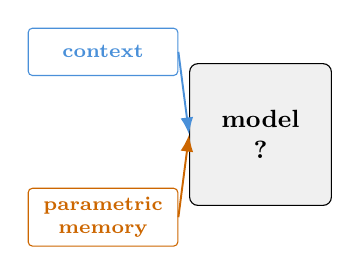
\begin{tikzpicture}[
  >=Latex,
  source/.style={draw, rounded corners=1.5pt, minimum width=19mm,
    minimum height=6mm, font=\scriptsize\bfseries, align=center},
  model/.style={draw, rounded corners=3pt, fill=lightgray,
    minimum width=18mm, minimum height=18mm, font=\small\bfseries,
    align=center}
]
  \node[source, draw=accentblue, text=accentblue] (ctx) at (0,1.05)
    {context};
  \node[source, draw=orange!80!black, text=orange!80!black] (mem) at (0,-1.05)
    {parametric\\memory};
  \node[model] (model) at (2.0,0) {model\\?};
  \draw[->, accentblue, line width=.7pt] (ctx.east) -- (model.west);
  \draw[->, orange!80!black, line width=.7pt] (mem.east) -- (model.west);
\end{tikzpicture}
\caption{\footnotesize A model must arbitrate between conflicting sources.}
\vspace{-5pt}
\end{wrapfigure}

When retrieved context contradicts a model's parametric memory, a small set of attention heads can be used, at test time, to steer whose word the model trusts \citep{li2025taming}. This paper asks whether that residual-stream geometry is an FP16 object or a property of the model that survives compression: if JuICE is computed on FP16, does it still steer after GPTQ INT4, even on items whose facts survive quantization? Accuracy can fall from forgetting, terse decoding, or a change in source arbitration; a transferred intervention distinguishes those cases. Figure~1 illustrates the underlying arbitration question; our test identifies causal heads on FP16, verifies them by dual-run steering, then applies the locked heads to GPTQ INT4, on Llama-3.1-8B and Gemma-2-9B base \citep{grattafiori2024llama,team2024gemma2}, after a behavioral check on Llama Instruct.

The contribution is a causal, head-level transfer test under GPTQ INT4 \citep{frantar2023gptq}, not a new accuracy table. After a question-aware matcher audit, Llama's published context-K10 transfer is a wrap artifact, while the locked parametric pair (clean K2) survives at $n{=}100$ on both precisions under gold-PAR-only counting. On Gemma, the published raw peak L27\_H6 is the same wrap; identified context-suppression $H^{-}$ versus a locked random-$K$ control, and a small context-K10 enlarge, survive entity confirmation at $n{=}100$. Behavioral efficacy is not, by itself, evidence that the same causal object survived compression.

Concretely, we show:
\begin{enumerate}
\item On Llama-3.1-8B-Instruct, GPTQ INT4 preserves closed-book recall on a double-filtered set while shifting conflict arbitration toward context (MR$^\star$ $-23.8$~pp $[-31.7,-17.1]$; cluster-robust AME $+10.3$~pp $[+3.1,+17.5]$).
\item On Llama-3.1-8B base, FP16 context K10 transfer ($+15$ $[+8,+23]$ under the original matcher) is a same-entity wrap: question-aware $\Delta$ is $+1$ $[+0,+3]$ (null) on INT4 and $+4$ $[+0,+8]$ (null) on FP16, against random-K10 $+0$ $[-4,+4]$ / $-1$ $[-4,+2]$. Native INT4 K10 leaves a thin leftover ($+4$ $[+1,+8]$). Reverse transfer is mostly a scorer artifact. The locked parametric pair survives at $n{=}100$ under gold-PAR-only counting ($-8$ $[-14,-3]$ on FP16; $-7$ $[-12,-2]$ on INT4).
\item On Gemma-2-9B base, directional ranking again buries the raw parametric peak, but that peak (L27\_H6) is a wrap artifact after the audit (hard zero at $n{=}50$; $+0$ $[-3,+3]$ at $n{=}100$ INT4). Two objects survive at $n{=}100$: identified $H^{-}$ versus random $K$ (inclusive $-19$ vs.\ $-1$ on FP16; $-11$ vs.\ $-1$ on INT4; gold-PAR-only $-15$ / $-10$), and a small context-K10 enlarge ($+7$ $[+2,+12]$ / $+5$ $[+1,+9]$).
\item The transferable object is therefore family-specific among the cells that were run. Gemma clean-K2 INT4 transfer was not run, so that missing cell is not evidence of non-transfer. Quantization-selectivity is not a universal ``context lives / parametric dies'' rule, and circuit claims require a matcher that cannot be gamed by role-phrase wrapping. A matched random-head control exists for Llama context K10 and Gemma $H^{-}$; none exists for the Llama $n{=}100$ clean-K2 headline.
\end{enumerate}

\section{Related Work}
\label{sec:related}

When retrieved context contradicts parametric memory, a language model must decide whose word to trust \citep{xie2024adaptive}. JuICE \citep{li2025taming} is a test-time, training-free dual-run intervention on a small set of attention heads. The original JuICE models are base checkpoints, not Instruct, a distinction developed in Methods (\S\ref{sec:instruct-base}). We do not revive a memory-head versus context-head dichotomy \citep{jin2024tug}; the transfer test is whether a locked intervention remains the same causal object after GPTQ. Prior compression work measures recall without a conflicting passage \citep{wang2026compressed} or RAG accuracy without constructed conflicts \citep{yazan2024rag}. Neither tests whether an FP16-identified arbitration intervention still acts on the same object after INT4. A drop in closed-book recall, or a stable RAG score, can occur without that circuit surviving. We double-filter on facts that remain answerable at both precisions and then transfer locked JuICE.

\section{Methods}
\label{sec:methods}

\subsection{Study scope and checkpoints}

Stage~1 is behavioral (Llama-3.1-8B-Instruct); Stage~2 is identify-and-steer on Llama-3.1-8B base and Gemma-2-9B base \citep{team2024gemma2,grattafiori2024llama}. Table~\ref{tab:models} lists every file. The Instruct INT4 artifact is a third-party community GPTQ, whereas the base INT4 artifacts are self-quantized; these are distinct files. Gemma has no Stage~1 Instruct GPTQ. Throughout, $n$ denotes the number of evaluation items, while $N_{\mathrm{CALIB}}$ denotes the GPTQ calibration-set size.

\begin{table}[H]
\caption{Checkpoints used in this paper. Rows are parallel across the two model families; “not run” marks the absent Gemma Stage~1 behavioral condition.}
\label{tab:models}
\centering
\scriptsize
\setlength{\tabcolsep}{3pt}
\begin{tabular}{p{1.15in}p{0.95in}p{0.7in}p{2.15in}}
\toprule
Role & Model & Precision & Checkpoint \\
\midrule
Stage~1 behavioral & Llama-3.1-8B-\textbf{Instruct} & FP16 & \path{meta-llama/Llama-3.1-8B-Instruct} \\
Stage~1 behavioral & Llama-3.1-8B-\textbf{Instruct} & GPTQ-INT4 & \path{hugging-quants/Meta-Llama-3.1-8B-Instruct-GPTQ-INT4} (third-party) \\
Stage~2 ID + steer & Llama-3.1-8B \textbf{base} & FP16 & \path{meta-llama/Llama-3.1-8B} \\
Stage~2 transfer (headline) & Llama-3.1-8B \textbf{base} & GPTQ-INT4 & self-quantized \path{llama31_8b_base_gptq_int4_ncalib128} ($N_{\mathrm{CALIB}}{=}128$) \\
Stage~2 robustness / native ID / recovery & Llama-3.1-8B \textbf{base} & GPTQ-INT4 & self-quantized \path{llama31_8b_base_gptq_int4} ($N_{\mathrm{CALIB}}{=}64$; retained for comparison) \\
Stage~1 behavioral & Gemma-2-9B \textbf{base} & not run & --- \\
Stage~2 ID + steer & Gemma-2-9B \textbf{base} & FP16 & \texttt{google/gemma-2-9b} \\
Stage~2 transfer (headline) & Gemma-2-9B \textbf{base} & GPTQ-INT4 & self-quantized \path{gemma2_9b_base_gptq_int4_ncalib128} ($N_{\mathrm{CALIB}}{=}128$) \\
\bottomrule
\end{tabular}
\end{table}
\FloatBarrier

\subsection{Instruct versus base mechanistic target}
\label{sec:instruct-base}

JuICE was developed on base models \citep{li2025taming}. We use $\texttt{dir\_par}=\texttt{par\_pos}-\texttt{ctx\_pos}$ as the directional parametric score. On Instruct with a chat template, parametric ID and steering fail (Table~\ref{tab:instruct-base}): this score is suppressed by $\sim$1130$\times$. This is a model-plus-prompt confound, so all INT4 transfer cells use base-identified heads.

\begin{table}[t]
\caption{Instruct (chat template) versus base (plain JuICE prompts). Parametric directional ID is suppressed on Instruct. Cell-3 numbers are from the original matcher; QA FP16 context K10 is $+4$ $[+0,+8]$.}
\label{tab:instruct-base}
\centering
\footnotesize
\setlength{\tabcolsep}{3pt}
\begin{tabular}{p{2.05in}cc}
\toprule
Metric (unit) & Instruct (chat) & Base (plain JuICE prompts) \\
\midrule
Raw enlarge Jaccard (unitless) & $\mathbf{0.54}$ & $\mathbf{0.053}$ \\
Peak raw \texttt{scores\_pos} (score units; ctx / par) & $0.0080$ / $0.0077$ & $\mathbf{0.036}$ / $\mathbf{0.058}$ \\
Best \texttt{dir\_par} (score units) & $\mathbf{2.68\times 10^{-4}}$ & $\mathbf{0.304}$ ($\sim$1130$\times$) \\
Directional top-10 Jaccard (unitless) & $0$ & $0$ \\
Parametric Cell-3 at $\alpha{+}{=}1$ (pp) & $0$ / $-2$ ($K{=}2$ / $K{=}3$) & $\mathbf{-6}$ to $\mathbf{-8}$ \\
Context Cell-3 at $\alpha{+}{=}1$ (pp) & $+6$ to $+8$ & $+6$ to $+10$ \\
\bottomrule
\end{tabular}
\end{table}

FP16 base must steer before transfer. Table~\ref{tab:fp16-gate} reports question-aware context K10 at $+4$ $[+0,+8]$ (null) and clean K2 at gold-PAR-only $-8$ $[-14,-3]$ (inclusive $-15$ $[-22,-7]$); those locked heads are then applied to INT4 without re-identification.

\subsection{GPTQ recipe and evaluation}

Stage~2 GPTQ uses gptqmodel 2.2, transformers 4.51.3, 4-bit quantization, group size 128, $\texttt{sym}{=}\texttt{True}$, and $\texttt{desc\_act}{=}\texttt{True}$. C4 is truncated to 512 tokens, with headline $N_{\mathrm{CALIB}}{=}128$; Llama $N_{\mathrm{CALIB}}{=}64$ is a robustness check only. Gemma uses the same recipe with \texttt{GetHeadsGemma2Attention} (GQA $16/8$, $\texttt{head\_dim}{=}256$, logit softcap $50$), eager attention, gptqmodel \texttt{BACKEND.TORCH}, and greedy $T{=}0$. Data is ConflictQA popular \citep{xie2024adaptive}. Stage~1 double-filters $n{=}250$ to $n{=}164$ items correct in closed-book mode at both precisions. Stage~2 uses the seed-42 $n{=}100$ IDs for Llama headline and diagnostic cells and for Gemma headlines; Gemma $n{=}50$ is a robustness check. Reverse-transfer cells remain on the original $n{=}50$ IDs. Head identification uses $|\mathcal{D}|{=}4$ shared calibration IDs, three-type JuICE completions, and $\texttt{FAST\_POS\_ALPHAS}{=}(1,3,5)$ and $\texttt{FAST\_NEG\_ALPHAS}{=}(-1,-2)$.

\subsection{JuICE intervention and scoring}

Steering is applied at decode time by dual-run JuICE (Figure~\ref{fig:juice-dualrun}), not by fine-tuning.
\begin{figure}[h]
\centering
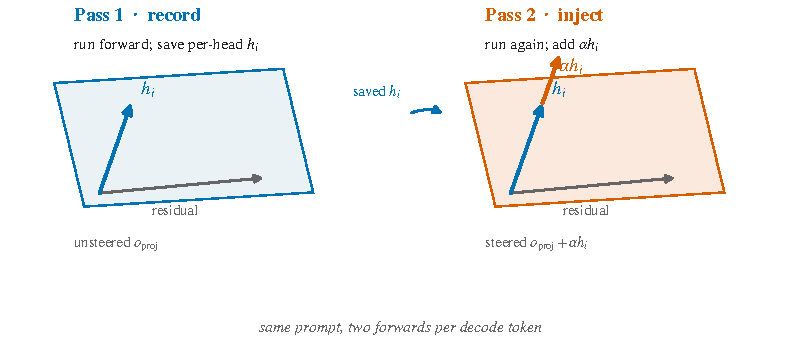
\includegraphics[width=0.55\linewidth]{figures/fig1_juice_dualrun.pdf}
\caption{Dual-run JuICE. Pass 1 records $h_i$ after \texttt{o\_proj}; pass 2 injects $\alpha h_i$.}
\label{fig:juice-dualrun}
\end{figure}
Pass 1 records per-head outputs after \texttt{o\_proj}; pass 2 adds $\alpha$ times the saved vector. We use context sets with $K{=}10$, parametric sets with clean/noisy $K{=}2$ and $K{=}3$, and $K{=}1$ on Gemma's raw parametric peak. Default transfer is enlarge-only, $\alpha{+}{=}1$, $\alpha{-}{=}0$; suppression uses $\alpha{+}{=}0$, $\alpha{-}{=}1$. Evaluation uses greedy \texttt{juice\_coherent} decoding with $\texttt{max\_new\_tokens}{=}16$. The output labels are \texttt{parametric}, \texttt{context}, \texttt{rejects\_context}, and \texttt{other}; we define \texttt{follows\_context} as the event that the label equals \texttt{context}. Here, $H^{-}$ denotes a suppression intervention with $\alpha_{+}{=}0$ and $\alpha_{-}{=}1$, and \texttt{exam-meta} denotes the multiple-choice-format text sometimes appended to a context-entity answer. A letter heuristic stayed at 100\% while $\alpha{=}3/5$ \texttt{other} hit 59--66\% on the $n{=}100$ question-aware grid (Table~\ref{tab:alpha-grid}), so we report label counts. Scorer brevity and parametric-first behavior are documented in Appendix~\ref{app:reverse}.

\subsection{Question-aware matching and gold-PAR-only counting}
\label{sec:matcher}

Stage~1 already passed \texttt{question=} into \texttt{label\_conflict\_response}. Stage~2 originally did not. Without the question, the matcher checks parametric gold first, including role-phrase aliases. Completions that assert the \emph{context} entity in a role frame (``Edina is the capital of Namibia'') were therefore labeled parametric. Passing the gold question strips echoed question tokens and relabels those wraps as context.

We report two $\Delta$ conventions after that audit. Inclusive $\Delta$ counts every baseline-context item that leaves the context label under steering. Gold-PAR-only $\Delta$ counts a leave-context move as success only when the steered completion mentions the gold parametric entity; leave-other and wrap items remain suppressed. Llama clean K2 uses gold-PAR-only as the conservative headline; inclusive $\Delta$ is an upper bound. Gemma identified $H^{-}$ headlines report inclusive $\Delta$ ($-19$ / $-11$); gold-PAR-only $\Delta$ is $-15$ / $-10$ (Table~\ref{tab:gemma-hminus-n50-n100}). Context-enlarge cells use inclusive $\Delta$ plus a same-entity wrap count. All Stage~2 $\Delta$ and CIs in Results are question-aware unless an original-matcher number is marked as such.

Paired bootstrap, 1000 draws, seed 42, percentile 95\% CI, throughout. Stage~1 resamples 164 items. Llama Stage~2 $\Delta$ is steered minus baseline \texttt{follows\_context} on 100 eval IDs; Gemma headlines use 100, with $n{=}50$ as robustness. Reverse transfer uses 50. ``Excludes 0'' is the detection rule. CIs are whole percentage points; gold-PAR-only n=100 FP16 K2 reports $[-14,-3]$ (bootstrap hi $-2.975$). Random-$K$ excludes the FP16 identified set. Gemma suppress specificity is $\Delta_{\mathrm{id}}-\Delta_{\mathrm{random}}$; DiD is $\mathrm{spec}_{INT4}-\mathrm{spec}_{FP16}$. We do not infer specificity from overlapping cell CIs.

The pre-registered Llama gate required same-sign transfer of context K10 and parametric clean K2 at coherence $\ge 0.90$ under the original matcher; that gate passed. The question-aware audit later nulls context K10 transfer and leaves clean K2 as the Llama headline. Gemma headlines are identified $H^{-}$ versus random $K$ and context K10 enlarge at $n{=}100$; L27\_H6 is a wrap artifact. The scope of unrun cells is consolidated in Limitations.

\section{Results}
\label{sec:results}

\subsection{Stage 1: behavioral arbitration on Instruct}
\label{sec:stage1}

Stage~1 asks, before any head is identified: when a fact survives INT4, does conflict arbitration still look like FP16? We compare FP16 Instruct to a third-party GPTQ-INT4 Instruct checkpoint on 250 ConflictQA popular items, then restrict to the 164 items closed-book correct at both precisions.

\begin{table}[t]
\caption{Stage~1 memorization rate. MR$^\star$ is the primary behavioral estimand (shared 164).}
\label{tab:mrstar}
\centering
\small
\begin{tabular}{lccc}
\toprule
Precision & Closed-book & MR (unfiltered) & MR$^\star$ (shared 164) \\
\midrule
FP16 & 182/250 (72.8\%) & 92/250 (36.8\%) & \textbf{76/164 (46.3\%)} \\
INT4 & 175/250 (70.0\%) & 48/250 (19.2\%) & \textbf{37/164 (22.6\%)} \\
\bottomrule
\end{tabular}
\end{table}

MR$^\star$ on the shared 164 is the primary estimand (Table~\ref{tab:mrstar}). It falls by $-23.8$~pp $[-31.7,-17.1]$ after quantization, excluding zero. Closed-book performance is nearly stable ($-7$ items), whereas unfiltered MR falls by $-17.6$~pp, so the arbitration shift does not disappear under the double filter. Cluster-robust logit AME on \texttt{follows\_context} is $+10.3$~pp $[+3.1,+17.5]$ (Table~\ref{tab:ame}); corrected label counts in Appendix Tables~\ref{tab:labels}--\ref{tab:transitions} show a parametric collapse and a rise in context. A first-pass substring scorer inflated the AME to $+20.6$~pp by counting denials as context, so it is not used here. Llama-3.2-1B-Instruct was a null screen and is not mixed into the 8B claim.

\begin{table}[t]
\caption{Stage~1 \texttt{follows\_context} AME on the shared 164 items. The cluster-robust logit row is the published estimand.}
\label{tab:ame}
\centering
\small
\begin{tabular}{lccc}
\toprule
Estimand & Point & 95\% CI & excl.\ 0? \\
\midrule
Cluster-robust logit AME & $\mathbf{+10.3}$~\textbf{pp} & $\mathbf{[+3.1, +17.5]}$ & yes \\
Raw $\Delta P(\texttt{context})$ & $+10.4$~pp & $(52{\to}69)/164$ & --- \\
Item-averaged AME & $+9.8$~pp & --- & --- \\
Mixed VB AME & $+16.1$~pp & $[+5.9, +26.2]$ & yes \\
\bottomrule
\end{tabular}
\end{table}

\begin{table}[t]
\caption{FP16 base steering on the 100 Llama eval items, question-aware matcher. Gold-PAR-only $\Delta$ for clean K2 counts only CTX$\to$gold-PAR-name flips; inclusive $\Delta$ is an upper bound. Letter heuristic coherence is 100\% in every row (not shown).}
\label{tab:fp16-gate}
\centering
\footnotesize
\setlength{\tabcolsep}{3pt}
\begin{tabular}{lccccc}
\toprule
Condition & Heads & $fc$ & $\Delta$ [95\% CI] & P/C/O \\
\midrule
baseline & --- & 67\% & --- & 23/67/10 \\
context K10 & directional ctx top-10 & 71\% & $+4$ $[+0,+8]$ (null) & 17/71/12 \\
parametric clean K2 (incl.) & \textbf{L20\_H14, L26\_H15} & 52\% & $-15$ $[-22,-7]$ & 31/52/17 \\
parametric clean K2 (gold-PAR) & same pair & --- & $\mathbf{-8}$ $\mathbf{[-14,-3]}$ & 9 gold-PAR / 7 leave \\
random context K10 & seed 42 & 67\% & $+0$ $[-4,+4]$ & 19/67/14 \\
\bottomrule
\end{tabular}
\end{table}

\subsection{Llama context K10 is a wrap artifact}
\label{sec:ctx-transfer}

On the expanded Llama set, original-matcher context K10 was $+8$ $[+2,+14]$ on FP16 and $+15$ $[+8,+23]$ in forward transfer to INT4. After the question-aware audit both cells are null: $+4$ $[+0,+8]$ on FP16 and $+1$ $[+0,+3]$ on INT4 (Table~\ref{tab:ctx-k10}, Figure~\ref{fig:deltas}). Random-K10 is $+0$ $[-4,+4]$ on FP16 and $-1$ $[-4,+2]$ on INT4. Entity audit of the original INT4 transfer flips finds 17/17 same-entity wraps: the steered completion still names the context entity in a role frame that the parametric-first matcher had scored as parametric. Native INT4 K10 remains a thin leftover ($+4$ $[+1,+8]$; about three real CTX switches among 17 wraps). We do not treat wrap-corrected context enlarge as a transferred circuit.

\begin{figure}[t]
\centering
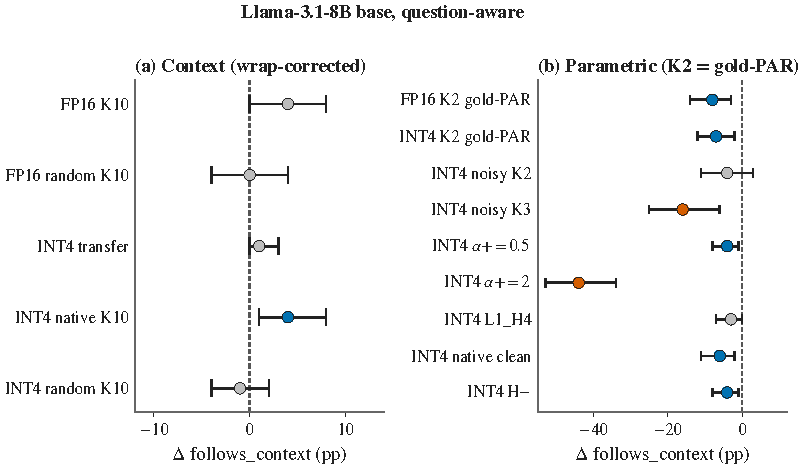
\includegraphics[width=\linewidth]{figures/fig2_delta_follows_context.pdf}
\caption{$\Delta$ \texttt{follows\_context} on 100 items after the question-aware audit (1000 paired draws, seed 42; $N_{\mathrm{CALIB}}{=}128$ for INT4). (a)~Context interventions, wrap-corrected. (b)~Parametric interventions: clean K2 uses gold-PAR-only $\Delta$; $\alpha{=}2$ (orange) is \texttt{other}-inflation, and $\alpha{=}3/5$ collapse to $-70$ is omitted. Blue-teal: CI excludes 0; grey: includes 0; orange: detected but inflated.}
\label{fig:deltas}
\end{figure}

\begin{table}[t]
\caption{Forward transfer of FP16 context K10 onto canonical INT4 ($\mathrm{N_{CALIB}{=}128}$), question-aware matcher. This cell is a wrap artifact (see \S\ref{sec:ctx-transfer}); original-matcher INT4 K10 was $+15$ $[+8,+23]$.}
\label{tab:ctx-k10}
\centering
\footnotesize
\setlength{\tabcolsep}{2.5pt}
\begin{tabular}{lcccccc}
\toprule
Condition & INT4 $fc$ & INT4 $\Delta$ [95\% CI] & excl.\ 0? & FP16 $\Delta$ [CI] & P/C/O \\
\midrule
baseline & 74\% & --- & --- & 67\% & 11/74/15 \\
\textbf{context K10} & 75\% & $+1$ $[+0,+3]$ & no & $+4$ $[+0,+8]$ & 9/75/16 \\
random context K10 & 73\% & $-1$ $[-4,+2]$ & no & $+0$ $[-4,+4]$ & 10/73/17 \\
native INT4 K10 & 78\% & $+4$ $[+1,+8]$ & yes & --- & 8/78/14 \\
\bottomrule
\end{tabular}
\end{table}

\subsection{Reverse transfer and native in-precision identification}
\label{sec:reverse}

Native INT4 context K10 applied in-precision (Cell~B) is the thin leftover above ($+4$ $[+1,+8]$). Reverse transfer of those heads onto FP16 (Cell~A, $n{=}50$) is mostly a scorer artifact: entity-confirmed detection persists at $\alpha{=}0.5$ ($+12$ $[+2,+24]$, 6 real CTX) but not at $\alpha{=}1$ ($+8$ $[-2,+20]$, null) or $\alpha{=}0.25$ ($+10$ $[+0,+20]$, null despite 6 real CTX) --- we do not treat this as a stable bidirectional effect. The original-matcher $\alpha$-sweep and the question-aware table are in Appendix~\ref{app:reverse}.

\subsection{Llama parametric clean K2 survives gold-PAR-only counting}
\label{sec:parametric}

FP16 clean K2 remains detected at $n{=}100$ when success is restricted to gold parametric names: $-8$ $[-14,-3]$ (9 CTX$\to$gold-PAR; 7 leave-without-PAR). Inclusive $\Delta$ is an upper bound ($-15$ $[-22,-7]$). The identical locked pair on INT4 is $-7$ $[-12,-2]$ gold-PAR-only (7 / 5) against inclusive $-12$ $[-19,-6]$. At $n{=}50$, gold-PAR-only FP16 is $-6$ $[-14,+0]$ (null) while INT4 $N_{\mathrm{CALIB}}{=}128$ is $-8$ $[-16,-2]$ (detected); we therefore treat $n{=}100$ as the headline (Table~\ref{tab:parametric-n50-n100}). Noisy K2 is $-4$ $[-11,+3]$ (null); noisy K3 is $-16$ $[-25,-6]$ with 28\% \texttt{other} and is not a recovered parametric object. Native clean K2 is $-6$ $[-11,-2]$; L1\_H4 is $-3$ $[-7,+0]$ (null). H$^-$ is $-4$ $[-8,-1]$. The $\alpha$ grid on the same pair is $-4$ $[-8,-1]$ at $0.5$, $-12$ $[-19,-6]$ at $1$, and $-44$ / $-70$ at $2$--$5$ with 36--66\% \texttt{other}: high-gain detections are scorer collapse. A random parametric-K2 file exists only at $n{=}50$ on the $N_{\mathrm{CALIB}}{=}64$ checkpoint, using L13\_H2 and L16\_H20 (seed 44; original-matcher $+4$ $[+0,+10]$). That is not a matched control for the locked L20\_H14+L26\_H15 headline at $n{=}100$, $N_{\mathrm{CALIB}}{=}128$; no such matched random-K2 cell was run.

\begin{table}[t]
\caption{Llama parametric clean-K2 expansion, question-aware matcher. Gold-PAR-only $\Delta$ is the conservative headline; inclusive $\Delta$ counts every leave-context move. All runs use seed 42 and 1000 paired draws.}
\label{tab:parametric-n50-n100}
\centering
\scriptsize
\setlength{\tabcolsep}{2pt}
\begin{tabular}{lcccc}
\toprule
Condition & $n{=}50$ gold-PAR & $n{=}100$ gold-PAR & $n{=}100$ incl. & excl.\ 0? \\
\midrule
FP16 clean K2 & $-6$ $[-14,+0]$ & $\mathbf{-8}$ $\mathbf{[-14,-3]}$ & $-15$ $[-22,-7]$ & yes \\
INT4 clean K2 transfer & $-8$ $[-16,-2]$ & $\mathbf{-7}$ $\mathbf{[-12,-2]}$ & $-12$ $[-19,-6]$ & yes \\
\bottomrule
\end{tabular}
\end{table}

\subsection{Directional re-ranking has a blind spot}
\label{sec:blindspot}

The parametric repairs above used directional ranking, $\texttt{directional\_par} := \texttt{par\_pos} - \texttt{ctx\_pos}$.
\begin{figure}[t]
\centering
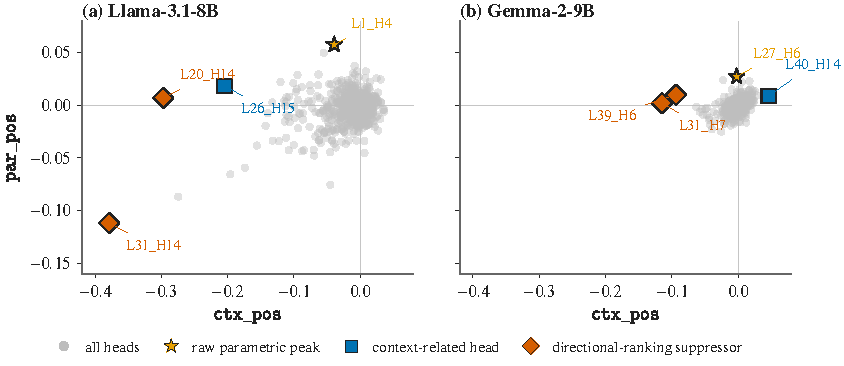
\includegraphics[width=\linewidth]{figures/fig_combined_identification.pdf}
\caption{FP16 identification scatter for Llama-3.1-8B and Gemma-2-9B on a shared axis scale. Light-gray points are all heads. Gold stars mark raw parametric peaks, blue-teal squares context-related heads, and coral diamonds directional-ranking suppressors; marker size and shape reinforce the role encoding.}
\label{fig:blindspot}
\end{figure}
\begin{flushleft}
That score can promote heads that suppress context tokens a lot, via a large negative $\texttt{ctx\_pos}$, over heads that actually boost parametric tokens (Figure~\ref{fig:blindspot}, Table~\ref{tab:blindspot}). The INT4 noise proxy, median $\max(|\texttt{ctx}|,|\texttt{par}|)$, is $9.2\times 10^{-3}$, so the $5\times$ threshold is $0.046$. Only L1\_H4 in or near the top 20 clears that threshold with positive $\texttt{par\_pos}$. Directional top-$K$ is therefore not interchangeable with the raw parametric peak without checking the sign of \texttt{par\_pos}.
\end{flushleft}

\begin{table}[t]
\caption{Directional re-ranking vs.\ raw parametric enlarge. L1\_H4 is the raw peak on both precisions and is ranked \#29 / \#14 by \texttt{dir\_par}.}
\label{tab:blindspot}
\centering
\footnotesize
\setlength{\tabcolsep}{2.5pt}
\begin{tabular}{p{0.55in}p{1.15in}p{1.7in}p{1.7in}}
\toprule
Head & Role & FP16 $\texttt{par\_pos}$ / $\texttt{ctx\_pos}$ / \texttt{dir\_par} (rank) & INT4 $\texttt{par\_pos}$ / $\texttt{ctx\_pos}$ / \texttt{dir\_par} (rank) \\
\midrule
\textbf{L1\_H4} & raw parametric enlarge \textbf{\#1} on both precisions & $\mathbf{+0.0577}$ / $-0.0392$ / $+0.0969$ (\textbf{\#29}) & $\mathbf{+0.0578}$ / $-0.0581$ / $+0.1159$ (\textbf{\#14}) \\
L20\_H14 & directional \#1; in clean + noisy K2 & $+0.0072$ / $-0.297$ / $\mathbf{+0.304}$ (\textbf{\#1}) & $\mathbf{-0.0436}$ / $-0.301$ / $+0.257$ (\textbf{\#1}) \\
L31\_H14 & noisy K2 (ctx-suppression) & $-0.112$ / $-0.378$ / $+0.267$ (\#2) & $-0.104$ / $-0.360$ / $+0.256$ (\#2) \\
L26\_H15 & clean K2 & $+0.0184$ / $-0.205$ / $+0.223$ (\#3) & $-0.0019$ / $-0.185$ / $+0.183$ (\#4) \\
\bottomrule
\end{tabular}
\end{table}

\subsection{Gemma-2-9B: identified $H^{-}$ and a small context-K10 enlarge}
\label{sec:model2}

We repeat identify$\times$apply on Gemma-2-9B \citep{team2024gemma2} with the same GPTQ recipe. Headlines use $n{=}100$; $n{=}50$ is robustness. Figure~\ref{fig:cross-family} summarizes the contrast after the audit: Llama's surviving object is clean K2; Gemma's are identified $H^{-}$ versus random $K$ and a small context enlarge. L27\_H6 does not survive. Figure~\ref{fig:gemma-deltas} and Tables~\ref{tab:gemma-fp16}--\ref{tab:gemma-hminus-n50-n100} report Gemma enlarge and $H^{-}$ results at $n{=}100$ (Appendix~\ref{app:gemma}).

\begin{figure}[t]
\centering
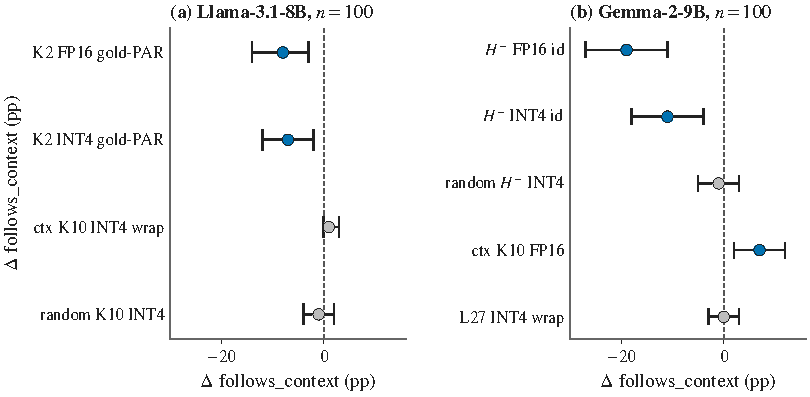
\includegraphics[width=\linewidth]{figures/fig6_cross_family.pdf}
\caption{Which object survives the question-aware audit, by family. Blue-teal: CI excludes 0; grey: includes 0. Llama K2 is gold-PAR-only; Gemma $H^{-}$ is inclusive $\Delta$ versus random $K$ at $n{=}100$. 1000 paired draws, seed 42.}
\label{fig:cross-family}
\end{figure}

Directional context-versus-parametric top-10 overlap is $0.0$. The clean parametric pair (L31\_H7, L39\_H6) consists of context suppressors, whereas L27\_H6 is the raw positive peak ($\texttt{par\_pos}{=}+0.027$; Figure~\ref{fig:blindspot}). Steering L27\_H6 is a wrap artifact: question-aware $\Delta$ is a hard zero at $n{=}50$ on both precisions and $+0$ $[-3,+3]$ at $n{=}100$ INT4 (Table~\ref{tab:gemma-fp16}). FP16 clean-K2 enlarge is detected at $n{=}100$ ($-6$ $[-12,-1]$); the INT4 transfer of that locked pair was not run and is not treated as a null. Context K10 enlarge, previously a ceiling null, is a small real effect at $n{=}100$: $+7$ $[+2,+12]$ on FP16 and $+5$ $[+1,+9]$ on INT4, against random-K10 $+0$ $[+0,+0]$ / $+3$ $[+0,+7]$.

Identified context-suppression $H^{-}$ is the Gemma headline. Inclusive $\Delta$ at $n{=}100$ is $-19$ $[-27,-11]$ on FP16 versus random $-1$ $[-5,+2]$, and $-11$ $[-18,-4]$ on INT4 versus random $-1$ $[-5,+3]$. Specificity is $-18$ $[-27,-10]$ / $-10$ $[-18,-2]$; DiD is $+8$ $[+1,+16]$ (FP16 specificity larger). Restricting success to gold parametric names---the same convention as Llama K2---leaves both $n{=}100$ identified cells detected: $-15$ $[-23,-8]$ on FP16 (16 gold-PAR / 4 leave) and $-10$ $[-17,-4]$ on INT4 (11 / 1). At $n{=}50$ the conservative count includes 0. Enlarge, $H^{-}$, and identification lists are detailed in Appendix~\ref{app:gemma}.

\section{Discussion}
\label{sec:discussion}

The two families reject a category-level account of transfer (Figure~\ref{fig:cross-family}). After the question-aware audit, Llama's surviving object at $n{=}100$ is the locked parametric pair under gold-PAR-only counting. Context K10 forward transfer is a wrap; native INT4 K10 is a thin leftover we do not promote to a circuit. Gemma's published raw peak L27\_H6 is the same wrap. The surviving Gemma objects are identified $H^{-}$ versus a locked random-$K$ control (gold-PAR-only still detected at $n{=}100$) and a small context-K10 enlarge. The evidence supports neither ``context survives compression'' nor ``parametric memory breaks.'' Rather, whether a particular causal object survives GPTQ is model- and direction-dependent, and depends on a matcher that cannot be gamed by role-phrase wrapping.

The cross-family regularity is methodological. In both families, the directional score $\texttt{par\_pos}-\texttt{ctx\_pos}$ elevates context suppressors above the strongest positive parametric signal. On Llama, checking the raw peak (L1\_H4) did not recover a useful INT4 parametric steer; on Gemma, checking it discovered the published wrap, not a transferable parametric object. Directional top-$K$ should therefore not be treated as interchangeable with a source-specific circuit without inspecting the underlying positive score, applying an intervention, and confirming the entity.

Our controls also separate an intervention effect from a circuit claim. Llama context K10 fails a wrap check that the original matcher passed. Gemma $H^{-}$ passes identified-versus-random at $n{=}100$ after the same check, including under gold-PAR-only counting. Reporting only the original-matcher cell would have overstated Llama context transfer and Gemma L27, and understated Gemma $H^{-}$. More generally, a same-sign output effect does not establish that the identified causal object, rather than a wrap or a generic intervention of the same size, survived compression.

% The former prospective second-model checklist was removed after completing Gemma-2.

\section{Conclusion}
\label{sec:conclusion}

If a source-arbitration intervention is computed in FP16 residual-stream geometry, GPTQ INT4 does not apply a uniform tax to that object. On Llama-3.1-8B base, the locked parametric pair survives at $n{=}100$ under gold-PAR-only counting, while context K10 transfer is a wrap artifact. On Gemma-2-9B base, identified $H^{-}$ versus random $K$ and a small context-K10 enlarge survive at $n{=}100$; L27\_H6 does not. The surviving object is therefore model-, direction-, and matcher-specific, not determined by source category. In both families, directional ranking promotes context suppressors over the strongest positive parametric signal, and a detected output effect is not the same as an entity-confirmed identified-versus-random contrast. Circuit-level claims about quantization therefore require the identify$\times$apply design, a matcher that cannot be gamed by role wrapping, a look at the completions, and a random-head control matched to the intervention---not a source label and a same-sign $\Delta$. Llama context K10 and Gemma $H^{-}$ have such a control; the Llama $n{=}100$ clean-K2 headline does not (the only random parametric-K2 result uses L13\_H2+L16\_H20 at $n{=}50$, $N_{\mathrm{CALIB}}{=}64$).

\section{Limitations}
\label{sec:limitations}

The following limitations define the scope of the claims.

The Llama expansion uses 100 held-out items, giving a 1~pp grid for proportions; Gemma headlines now use the same $n{=}100$ IDs, with $n{=}50$ as robustness. Reverse transfer remains $n{=}50$. The Llama clean-K2 gold-PAR-only transfer is $-7$ $[-12,-2]$ at $n{=}100$; the $n{=}50$ FP16 gold-PAR-only cell includes 0. Higher alpha produces scorer collapse, so we do not treat those larger deltas as stronger effects. Head identification remains thin at four calibration items.

The matcher audit is a post-hoc rescore of saved completions; original JSON labels were not rewritten. Stage~1 already passed \texttt{question=}; Stage~2 did not until this audit. Gold-PAR-only counting recodes leave-other and wrap as still-suppressed; item 1353 (steered ``General Aung San'') is human gold-PAR but missed by automatic mention after question-stripping and does not change detection. One native-K10 leftover involves a Tunis$\subset$Tunisia substring. Entity dumps are \texttt{entity\_audit\_k2\_k10.txt} and \texttt{entity\_audit\_hminus.txt}. Figures were redrawn from the same question-aware numbers as the text.

Head-set drift is not identifiable at this calibration size except as the observation that top-2 parametric is stable. Identification used four calibration items. Observed FP16-versus-INT4 overlap sits within the INT4-versus-INT4 noise floor for every spec we computed. Jaccard noise uses 25 draws. The quantization recipe is equally specific.

All INT4 results are GPTQ at 4-bit with group size 128. We did not test AWQ, bitsandbytes, or other recipes. Claims are about this GPTQ INT4 object, not about quantization in general. Even within that recipe, the unsteered baseline is not perfectly stable.

Unsteered INT4 \texttt{follows\_context} shifted from 14\% to 20\% between the $N_{\mathrm{CALIB}}{=}64$ and $N_{\mathrm{CALIB}}{=}128$ checkpoints on the same 50 eval ids under the original matcher. Steered deltas are paired against their own session's baseline. The two stages also do not share a weight file.

Stage~1 and Stage~2 use different INT4 artifacts: a third-party Instruct GPTQ versus a self-quantized base checkpoint. The headline Stage~2 calibration size is $N_{\mathrm{CALIB}}{=}128$; $N_{\mathrm{CALIB}}{=}64$ is retained for comparison. The cited recovery arms (the $\alpha$-grid, L1\_H4, noisy/native directional K2/K3, and H$-$) were run at $n{=}100$, $N_{\mathrm{CALIB}}{=}128$. Older $N_{\mathrm{CALIB}}{=}64$, $n{=}50$ copies of those arms exist as historical files and are not the numbers cited in Appendix~\ref{app:parametric}. Scoring choices further bound what those cells can say.

AME still uses equality to \texttt{``context''} only; breakdowns keep \texttt{rejects\_context}. The letter heuristic stayed at 100\% while $\alpha{=}3/5$ \texttt{other} hit 59--66\% on the $n{=}100$ question-aware grid (Table~\ref{tab:alpha-grid}), which is why we report label counts rather than the heuristic alone. The parametric-first / brevity pattern is a pipeline property of the scorer on \texttt{juice\_coherent} completions; the question-aware audit is the correction used in Results. Cluster-robust AME $+10.3$ $[+3.1, +17.5]$ is from the Stage~1 memo, not a re-fit in this writeup. The 1B null/confound screen is not mixed into the 8B claim. Instruct Cell-3 parametric $0/-2$~pp has no paired bootstrap.

The empirical scope is two base-model families, one GPTQ recipe, and conflict items from ConflictQA popular. Llama Stage~2 headline and diagnostic cells use 100 evaluation items; Gemma headlines use 100, with four head-identification calibration items per family. Gemma Stage~2 is base-only: there is no Gemma Instruct MR$^\star$, native INT4 re-identification, reverse transfer, or clean-K2 INT4 transfer, and those cells are not inferred from Llama. Gemma $H^{-}$ specificity excludes 0 at $n{=}100$ and includes 0 at $n{=}50$. These results are not claims about all LLMs, production RAG, or bidirectional circuit transfer.

\subsection*{Reproducibility statement}

(This section is recommended and does not count toward the page limit.)

Paired bootstrap is the detection protocol throughout. Stage~1 resamples the 164 double-filtered items; Llama Stage~2 resamples 100 eval items, while Gemma headlines resample 100 and Gemma robustness resamples 50. Both use 1000 draws and a percentile 95\% CI, with seed 42 throughout (random-$K$ additionally uses seeds 42--45). Decode is greedy at $T{=}0$. Head-identification calibration IDs, the eval split, locked head sets, and the GPTQ recipe ($\mathrm{N_{CALIB}}$, group size, \texttt{sym}, \texttt{desc\_act}) are specified in \S\ref{sec:methods}. Question-aware rescoring and gold-PAR-only counting are specified in \S\ref{sec:matcher}. Code and data will be released in anonymized form with the submission as anonymous supplementary material. This statement does not itself contain the reproduction recipe; the recipe is \S\ref{sec:methods}--\S\ref{sec:results}.

\subsection*{Notation}
\begin{center}
\footnotesize
\begin{tabular}{p{0.95in}p{4.2in}}
\toprule
$n$ & Number of evaluation items; Llama Stage~2 uses $n{=}100$; Gemma headlines use $n{=}100$ with $n{=}50$ robustness; reverse transfer uses $n{=}50$. \\
$N_{\mathrm{CALIB}}$ & GPTQ calibration-set size; headline $128$, robustness check $64$. \\
$K$ & Number of intervened heads; $K{=}10$ for context, $K{=}2$ for parametric pairs, and $K{=}1$ for Gemma's raw peak. \\
$H^{-}$ & Context-suppression intervention with $\alpha_{+}{=}0$ and $\alpha_{-}{=}1$. \\
$fc$ & \texttt{follows\_context}, the fraction labeled \texttt{context}. \\
$\texttt{ctx\_pos}$, $\texttt{par\_pos}$, $\texttt{dir\_par}$ & Context score, parametric score, and $\texttt{par\_pos}-\texttt{ctx\_pos}$ directional score. \\
\texttt{exam-meta} & Multiple-choice-format text appended to some context-entity completions; treated as a scorer artifact when diagnosed. \\
gold-PAR-only & Conservative $\Delta$: CTX$\to$leave counts as success only if the steered text mentions the gold parametric entity. \\
\bottomrule
\end{tabular}
\end{center}

\subsection*{AI use disclosure}
\label{sec:ai}

(This section is \textbf{required} and does not count toward the page limit.)

Cursor-based generative AI tools were used during implementation to draft and refactor analysis code, debug execution and LaTeX issues, generate and revise figure layouts, inspect rendered outputs, and edit manuscript language. The authors selected the experiments and evaluation protocol, ran and inspected the analyses, checked every reported result against saved outputs, and take responsibility for the methods, claims, interpretations, and conclusions.

\clearpage
\bibliography{references}
\bibliographystyle{iclr2027_conference}

\clearpage
\appendix

\section{Reverse transfer and native identification}
\label{app:reverse}

Forward transfer under the original matcher showed that FP16's context K10 still moved the scorer on INT4. After the question-aware audit that cell is a wrap. Native INT4 K10 applied in-precision remains a thin leftover ($+4$ $[+1,+8]$ on $n{=}100$). Reverse transfer of those heads onto FP16 (Cell~A) was run on the original $n{=}50$ IDs, $\alpha{+}{=}1$, $\alpha{-}{=}0$ unless noted, with the same paired bootstrap (1000 draws, seed 42). The native INT4 set is L7\_H26, L14\_H10, L7\_H21, L4\_H5, L3\_H3, L31\_H20, L4\_H11, L14\_H23, L8\_H29, L9\_H0. Jaccard versus FP16 K10 is $0.33$ (overlap 5/15: L7\_H26, L4\_H5, L31\_H20, L14\_H23, L9\_H0). Baselines are reused from prior sessions.

\begin{table}[h]
\caption{Identify$\times$apply triangulation for context K10. Original-matcher numbers are in parentheses. Cell~B is a thin leftover; Cell~A is not a stable reverse circuit.}
\label{tab:cells}
\centering
\footnotesize
\setlength{\tabcolsep}{2pt}
\begin{tabular}{lp{0.95in}ccp{1.7in}}
\toprule
Cell & Identify $\to$ apply & $fc$ (QA) & QA $\Delta$ [95\% CI] & Comparator \\
\midrule
\textbf{A reverse} ($n{=}50$) & INT4 K10 $\to$ FP16 & 76\% & $+8$ $[-2,+20]$ null & orig.\ $+48$ $[+34,+62]$; FP16-ID K10 on FP16 (QA): $+4$ $[+0,+8]$ \\
\textbf{B native} ($n{=}100$) & INT4 K10 $\to$ INT4 $N_{\mathrm{CALIB}}{=}128$ & 78\% & $+4$ $[+1,+8]$ yes & orig.\ $+16$ $[+8,+24]$; FP16-ID K10 on INT4 (QA): $+1$ $[+0,+3]$ \\
\bottomrule
\end{tabular}
\end{table}

Letter-heuristic coherence remained at 100\% in both cells. Cell~B is not a reproduction of the original $+16$ object: after wrap correction it is $+4$ $[+1,+8]$ with about three real CTX switches. Inspecting original-matcher \texttt{other} labels still shows terse names or short fragments, not the fluent rambling of high-alpha parametric collapse.

Cell~A is a rejected same-circuit hypothesis. Reverse transfer is mostly a scorer artifact: entity-confirmed detection persists at $\alpha{=}0.5$ ($+12$ $[+2,+24]$, 6 real CTX) but not at $\alpha{=}1$ ($+8$ $[-2,+20]$, null) or $\alpha{=}0.25$ ($+10$ $[+0,+20]$, null despite 6 real CTX) --- we do not treat this as a stable bidirectional effect. The original-matcher $\alpha$-sweep (Table~\ref{tab:cell-a-alpha}) recorded a large positive at every gain with exam-meta 36--58\%. Question-aware P/C/O is Table~\ref{tab:cell-a-alpha-qa}. On INT4's own ID, 9/10 of the native K10 heads are context-specific ($\texttt{ctx\_pos}{>}0$ and $\texttt{par\_pos}{\le}0$); L8\_H29 is the exception. Two INT4-only heads are context-negative when scored on FP16 ID. Steering that set on FP16 is not the same K10.

The scorer has a pipeline property that the question-aware matcher corrects. Some parametric-to-context flips occur when the unsteered baseline already named the context entity in a full sentence, labeled \texttt{parametric} because the matcher checks parametric gold first, and steering shortens the completion to a bare name that then labels \texttt{context}. We therefore report label counts, wrap counts, and gold-PAR-only $\Delta$ where the claim is parametric.

\section{Parametric recovery attempts: full detail}
\label{app:parametric}

On FP16, the clean K2 pair remains detected at $n{=}100$ under gold-PAR-only counting ($-8$~pp, $[-14,-3]$; 9 gold-PAR / 7 leave). Inclusive $\Delta$ is $-15$ $[-22,-7]$. On INT4, the identical locked pair is $-7$ $[-12,-2]$ gold-PAR-only (7 / 5) against inclusive $-12$ $[-19,-6]$. All diagnostic arms below use the $n{=}100$, $N_{\mathrm{CALIB}}{=}128$ reruns unless noted, question-aware.

\paragraph{0. Transfer of the FP16 clean pair.}
The starting test applies L20\_H14 and L26\_H15 at $\alpha{+}{=}1$, $\alpha{-}{=}0$. Inclusive INT4 $\Delta$ is $-12$ $[-19,-6]$ (P/C/O 18/62/20). Gold-PAR-only is the headline. The original-matcher $n{=}50$ result was the borderline $-4$ $[-10,0]$ null that motivated expansion.

\paragraph{1. Alpha grid on the same clean pair.}
If INT4 merely rescaled the same axis, a different $\alpha{+}$ should restore a cleaner object. Table~\ref{tab:alpha-grid} reports question-aware $\alpha{+} \in \{0.5, 1, 2, 3, 5\}$ with $\alpha{-}{=}0$ and $n{=}100$. The letter heuristic remains at 100\% at every gain. At $\alpha{=}3$ and $5$, \texttt{other} is 59--66\%: fluent-looking rambling, blank-slot, and off-entity completions, not parametric answers. The $-70$~pp detections at $\alpha{=}3/5$ are scorer collapse. Rescale does not restore a stronger parametric object.

\paragraph{2. L1\_H4, the raw parametric peak.}
L1\_H4 is the only INT4 (and FP16) head with $\texttt{par\_pos}$ above $5\times$ the identification noise floor. On the n=100 INT4 rerun, steering $K{=}1$ at $\alpha{+}{=}1$, $\alpha{-}{=}0$ yields $-3$ $[-7,+0]$, which includes 0; P/C/O is 14/71/15. The raw peak remains a null control rather than reproducing the clean-pair effect.

\paragraph{3. Native INT4 re-identification.}
The native clean filter returns L16\_H30 and L17\_H27. Applied on the $N_{\mathrm{CALIB}}{=}128$ checkpoint at $K{=}2$, $\alpha{+}{=}1$, $\alpha{-}{=}0$ on 100 items, this pair yields $-6$ $[-11,-2]$ (P/C/O 17/68/15). This is detected under inclusive counting and is not the locked FP16 pair.

\paragraph{4. Context-suppression as a parametric proxy.}
H$-$ is the FP16 directional context K10, enlarge empty, $\alpha{+}{=}0$, $\alpha{-}{=}1$. On 100 items the question-aware delta is $-4$ $[-8,-1]$, with P/C/O 16/70/14. This is a detected suppression proxy, not evidence that the parametric clean pair is stronger.

\paragraph{Jaccard vs.\ $|\mathcal{D}|{=}4$ noise.}
Head-set overlap is not identifiable at this calibration size. Twenty-five calibration-item resamples place every observed FP16-versus-INT4 Jaccard we computed within the INT4-versus-INT4 noise floor (context K10 $J{=}0.33$ versus noise mean $0.27$ $[0.05, 0.82]$; parametric K2 $J{=}1.0$ versus noise already about $0.95$). The exception, such as it is, is that top-2 parametric is stable. The Jaccard noise uses 25 draws.

Taken together, this is gold-PAR-only transfer of the locked pair at $n{=}100$, not a blanket parametric recovery. Higher-gain detections are accompanied by 36--66\% \texttt{other} outputs and are scorer collapse.

\section{Gemma-2-9B identification, transfer, and suppress-specificity}
\label{app:gemma}

Figure~\ref{fig:gemma-deltas} and Tables~\ref{tab:gemma-fp16}--\ref{tab:gemma-hminus-n50-n100} are the $n{=}100$ Gemma enlarge and $H^{-}$ displays cited from \S\ref{sec:model2}.

\begin{figure}[ht]
\centering
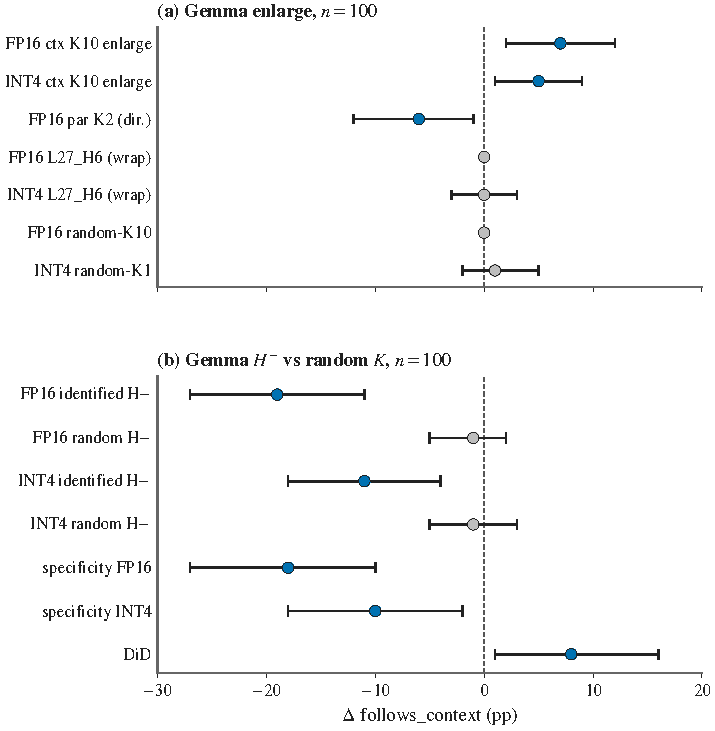
\includegraphics[width=\linewidth]{figures/fig5_gemma_deltas.pdf}
\caption{Gemma $\Delta$ \texttt{follows\_context} at $n{=}100$, question-aware. (a)~Context K10 enlarge is a small detected effect; L27\_H6 is a wrap zero. (b)~Identified $H^{-}$ versus random $K$; specificity and DiD exclude 0.}
\label{fig:gemma-deltas}
\end{figure}

\begin{table}[ht]
\caption{Gemma-2-9B enlarge cells after the question-aware audit. L27\_H6 is a wrap; context K10 enlarge is the small surviving enlarge. Clean-K2 INT4 transfer was not run. Letter heuristic 100\%.}
\label{tab:gemma-fp16}
\centering
\footnotesize
\setlength{\tabcolsep}{3pt}
\begin{tabular}{lcccc}
\toprule
Condition & Heads / notes & $n{=}50$ $\Delta$ [CI] & $n{=}100$ $\Delta$ [CI] & excl.\ 0 at $n{=}100$? \\
\midrule
FP16 ctx K10 enlarge & directional top-10 & $+4$ $[+0,+10]$ & $\mathbf{+7}$ $\mathbf{[+2,+12]}$ & yes \\
INT4 ctx K10 enlarge & same locked set & --- & $\mathbf{+5}$ $\mathbf{[+1,+9]}$ & yes \\
FP16 par K2 clean & L31\_H7, L39\_H6 & $-2$ $[-10,+4]$ & $-6$ $[-12,-1]$ & yes \\
INT4 par K2 clean & same locked pair & --- & not run & --- \\
FP16 L27\_H6 & raw peak & $+0$ $[+0,+0]$ & $+0$ $[+0,+0]$ & no \\
INT4 L27\_H6 & same locked head & $+0$ $[+0,+0]$ & $+0$ $[-3,+3]$ & no \\
INT4 random $K{=}1$ & L40\_H15 & $+0$ $[-6,+6]$ & $+1$ $[-2,+5]$ & no \\
FP16 random-K10 enlarge & seed 42 & $+0$ $[+0,+0]$ & $+0$ $[+0,+0]$ & no \\
\bottomrule
\end{tabular}
\end{table}

\begin{table}[ht]
\caption{Gemma identified $H^{-}$ versus locked random $K$. Inclusive $\Delta$ counts every leave-context move; gold-PAR-only $\Delta$ uses the Llama-K2 convention. $n{=}50$ is robustness.}
\label{tab:gemma-hminus-n50-n100}
\centering
\footnotesize
\setlength{\tabcolsep}{2pt}
\begin{tabular}{lcccc}
\toprule
Condition & $n{=}50$ incl.\ [CI] & $n{=}100$ incl.\ [CI] & $n{=}100$ gold-PAR [CI] & excl.\ 0 at $n{=}100$? \\
\midrule
FP16 identified H$-$ & $-14$ $[-26,-4]$ & $\mathbf{-19}$ $\mathbf{[-27,-11]}$ & $\mathbf{-15}$ $\mathbf{[-23,-8]}$ & yes \\
INT4 identified H$-$ & $-8$ $[-16,+0]$ & $\mathbf{-11}$ $\mathbf{[-18,-4]}$ & $\mathbf{-10}$ $\mathbf{[-17,-4]}$ & yes \\
FP16 random H$-$ & $-4$ $[-10,+0]$ & $-1$ $[-5,+2]$ & --- & no \\
INT4 random H$-$ & $-2$ $[-10,+4]$ & $-1$ $[-5,+3]$ & --- & no \\
specificity FP16 & $-10$ $[-22,+2]$ & $-18$ $[-27,-10]$ & --- & yes \\
specificity INT4 & $-6$ $[-18,+6]$ & $-10$ $[-18,-2]$ & --- & yes \\
DiD & $+4$ $[-4,+14]$ & $+8$ $[+1,+16]$ & --- & yes \\
\bottomrule
\end{tabular}
\end{table}

We repeat the base-model identify$\times$apply protocol on Gemma-2-9B using the same four calibration IDs, the same GPTQ recipe ($\mathrm{N_{CALIB}{=}128}$), and the same paired bootstrap. Headlines use $n{=}100$; $n{=}50$ is robustness. Native INT4 re-identification, reverse transfer, and clean-K2 INT4 transfer of L31\_H7+L39\_H6 were not run; those cells remain empty.

\paragraph{Identification.}
FP16 directional context and parametric top-10 sets are fully separated (Jaccard $0.0$; noise-proxy median $0.0063$). The directional context K10 is L40\_H14, L17\_H7, L24\_H15, L22\_H0, L32\_H11, L25\_H0, L3\_H9, L8\_H9, L7\_H6, L29\_H5. The directional / clean parametric $K{=}2$ pair is L31\_H7, L39\_H6---identical, and both are context suppressors ($\texttt{ctx\_pos}$ $-0.115$ / $-0.094$; $\texttt{par\_pos}$ $0.002$ / $0.010$, at or near the noise floor). They rank as parametric only because $\texttt{directional\_par} = \texttt{par\_pos} - \texttt{ctx\_pos}$ is large when $\texttt{ctx\_pos}$ is large-negative. The raw positive parametric peak is L27\_H6 ($\texttt{par\_pos}{=}+0.027$), the Llama L1\_H4 analog. Locked random-K10 heads (reused for suppress controls): L41\_H11, L7\_H3, L1\_H9, L17\_H13, L15\_H13, L14\_H7, L9\_H1, L6\_H9, L35\_H9, L5\_H10. Identification ranking is unchanged by the matcher audit; only the steered labels change.

\paragraph{L27\_H6 is a wrap.}
Original-matcher L27\_H6 was $-12$ on FP16 and $-8$ on INT4 at $n{=}50$. Question-aware $\Delta$ is a hard zero at $n{=}50$ on both precisions (1000/1000 draws exactly zero) and $+0$ $[-3,+3]$ at $n{=}100$ INT4. The published transfer was role-phrase wrapping of the same entity.

\paragraph{Context K10 enlarge is a small real effect at $n{=}100$.}
Question-aware context K10 enlarge is $+7$ $[+2,+12]$ on FP16 and $+5$ $[+1,+9]$ on INT4 at $n{=}100$, against random-K10 $+0$ $[+0,+0]$ / $+3$ $[+0,+7]$. At $n{=}50$ the FP16 cell is $+4$ $[+0,+10]$ (null). This is a small enlarge, not a Llama-style wrap-inflated $+15$.

\paragraph{Identified $H^{-}$ versus random $K$.}
Identified H$-$ is $-19$ $[-27,-11]$ on FP16 and $-11$ $[-18,-4]$ on INT4 at $n{=}100$ (inclusive). Locked random H$-$ is $-1$ on both precisions. Specificity and DiD exclude 0 at $n{=}100$ and include 0 at $n{=}50$ (Table~\ref{tab:gemma-hminus-n50-n100}). Gold-PAR-only $\Delta$ remains detected at $n{=}100$ ($-15$ / $-10$). We report this as the Gemma headline, not L27\_H6.

\section{Detailed diagnostic tables}
\label{app:diagnostics}

The historical $N_{\mathrm{CALIB}}{=}64$ versus $128$ comparison was run on the original 50-item set and is not repeated here; the expanded $n{=}100$ gold-PAR-only comparison is Table~\ref{tab:parametric-n50-n100}. Context K5 was run only at $n{=}50$ (FP16 and INT4 $N_{\mathrm{CALIB}}{=}64$) and was not expanded to the $n{=}100$ audit.

\begin{table}[h]
\caption{Cell~A $\alpha$-sweep, original matcher: INT4 K10 heads applied on FP16 ($n{=}50$). Exam-meta is the fraction of context labels with exam-meta dump. Kept for comparison with Table~\ref{tab:cell-a-alpha-qa}.}
\label{tab:cell-a-alpha}
\centering\small
\begin{tabular}{ccccccc}
\toprule
$\alpha{+}$ & $fc$ & $\Delta$ [95\% CI] & excl.\ 0? & Coh & exam-meta & P/C/O \\
\midrule
$0.25$ & 50\% & $\mathbf{+34}$ $\mathbf{[+20,+50]}$ & yes & 100\% & $\mathbf{58\%}$ & 21/25/4 \\
$0.5$ & 52\% & $\mathbf{+36}$ $\mathbf{[+22,+50]}$ & yes & 100\% & $\mathbf{52\%}$ & 18/26/6 \\
$1.0$ & 64\% & $\mathbf{+48}$ $\mathbf{[+34,+62]}$ & yes & 100\% & 36\% & 12/32/6 \\
\bottomrule
\end{tabular}
\end{table}

\begin{table}[h]
\caption{Cell~A $\alpha$-sweep, question-aware matcher: INT4 K10 heads applied on FP16 ($n{=}50$). Real CTX is the entity-confirmed context-entity switch count among QA flips. Baseline P/C/O $12/34/4$.}
\label{tab:cell-a-alpha-qa}
\centering\small
\begin{tabular}{cccccc}
\toprule
$\alpha{+}$ & $fc$ & $\Delta$ [95\% CI] & excl.\ 0? & real CTX & P/C/O \\
\midrule
$0.25$ & 78\% & $+10$ $[+0,+20]$ & no & 6 & 5/39/5 \\
$0.5$ & 80\% & $\mathbf{+12}$ $\mathbf{[+2,+24]}$ & yes & 6 & 4/40/5 \\
$1.0$ & 76\% & $+8$ $[-2,+20]$ & no & 5 & 4/38/5 \\
\bottomrule
\end{tabular}
\end{table}

\begin{table}[h]
\caption{Rescale repair: $\alpha$-grid on FP16 clean K2 applied to INT4 ($N_{\mathrm{CALIB}}{=}128$, $n{=}100$), question-aware matcher.}
\label{tab:alpha-grid}
\centering\small
\begin{tabular}{ccccc}
\toprule
$\alpha{+}$ & $\Delta$ [95\% CI] & excl.\ 0? & P/C/O & Coh heuristic \\
\midrule
$0.5$ & $-4$ $[-8,-1]$ & yes & 14/70/16 & 100\% \\
$1$ & $\mathbf{-12}$ $\mathbf{[-19,-6]}$ & yes & 18/62/20 & 100\% \\
$2$ & $\mathbf{-44}$ $\mathbf{[-53,-34]}$ & yes & 34/30/36 & 100\% \\
$3$ & $\mathbf{-70}$ $\mathbf{[-79,-60]}$ & yes & 37/4/59 & 100\%* \\
$5$ & $\mathbf{-70}$ $\mathbf{[-79,-61]}$ & yes & 30/4/66 & 100\%* \\
\bottomrule
\end{tabular}
\end{table}

\begin{table}[h]
\caption{Native INT4 parametric re-identification versus FP16, and question-aware apply results ($n{=}100$ where rerun).}
\label{tab:native-id}
\centering\footnotesize
\begin{tabular}{p{1.35in}p{1.15in}p{0.9in}p{1.4in}}
\toprule
Spec & INT4 set & versus FP16 & Apply result (QA) \\
\midrule
noisy par K2 & L20\_H14, L31\_H14 & Jaccard $\mathbf{1.0}$ & $-4$ $[-11,+3]$ null \\
noisy par K3 & L20\_H14, L31\_H14, L8\_H9 & $J{=}0.50$ & $-16$ $[-25,-6]$ (28\% other) \\
clean K2 & \textbf{L16\_H30, L17\_H27} & Jaccard $\mathbf{0.00}$ & $-6$ $[-11,-2]$; P/C/O 17/68/15 \\
L1\_H4 $K{=}1$ & raw peak & --- & $-3$ $[-7,+0]$ null \\
\bottomrule
\end{tabular}
\end{table}

\begin{table}[h]
\caption{Matcher-audit summary: original-matcher headline versus question-aware call. Wrap = same-entity role-phrase flip. For Llama K2, the original-matcher column is $n{=}100$ inclusive $\Delta$ (FP16 $-8$ $[-14,-3]$, INT4 $-4$ $[-8,-1]$), not gold-PAR-only and not the $n{=}50$ INT4 $N_{\mathrm{CALIB}}{=}128$ original-matcher cell $-4$ $[-10,+0]$. Gold-PAR-only is the conservative parametric $\Delta$.}
\label{tab:artifact-summary}
\centering\scriptsize
\setlength{\tabcolsep}{2pt}
\begin{tabular}{lp{1.15in}p{1.45in}p{0.95in}}
\toprule
Claim & Original matcher & Question-aware & Call after audit \\
\midrule
Llama INT4 ctx K10 & $+15$ $[+8,+23]$ & $+1$ $[+0,+3]$; 17/17 wrap & wrap artifact \\
Llama FP16 ctx K10 & $+8$ $[+2,+14]$ & $+4$ $[+0,+8]$; 4 real CTX & null \\
Llama native INT4 K10 & $+16$ $[+8,+24]$ & $+4$ $[+1,+8]$ & thin leftover \\
Llama K2 $n{=}100$ (FP16/INT4) & orig.\ incl.\ $-8$ $[-14,-3]$ / $-4$ $[-8,-1]$ & gold-PAR $-8$ $[-14,-3]$ / $-7$ $[-12,-2]$ & survives \\
Gemma L27\_H6 & $-12$ / $-8$ & hard $0$ / $+0$ $[-3,+3]$ & wrap artifact \\
Gemma $H^{-}$ $n{=}100$ & $-13$ / $-8$ vs random detected & $-19$ vs $-1$ / $-11$ vs $-1$; gold-PAR $-15$ / $-10$ & survives \\
Gemma ctx K10 $n{=}100$ & $+4$ / $+4$ null & $+7$ $[+2,+12]$ / $+5$ $[+1,+9]$ & small real \\
\bottomrule
\end{tabular}
\end{table}

\begin{table}[h]
\caption{Stage~1 label shift on the shared 164 items, corrected scorer.}
\label{tab:labels}
\centering\small
\begin{tabular}{lccc}
\toprule
Label & FP16 & INT4 & $\Delta$ \\
\midrule
parametric & 76 & 37 & $\mathbf{-39}$ \\
context & 52 & 69 & $\mathbf{+17}$ \\
\texttt{rejects\_context} & 13 & 22 & $+9$ \\
other & 23 & 36 & $+13$ \\
\bottomrule
\end{tabular}
\end{table}

\begin{table}[h]
\caption{Stage~1 FP16-to-INT4 label transitions on the shared 164 items, corrected scorer.}
\label{tab:transitions}
\centering\small
\begin{tabular}{lcccc}
\toprule
 & $\to$ parametric & $\to$ context & $\to$ \texttt{rejects\_context} & $\to$ other \\
\midrule
\textbf{parametric $\to$} & 33 & \textbf{20} & 10 & 13 \\
\textbf{context $\to$} & 3 & 41 & 5 & 3 \\
\textbf{\texttt{rejects\_context} $\to$} & 0 & 3 & 5 & 5 \\
\textbf{other $\to$} & 1 & 5 & 2 & 15 \\
\bottomrule
\end{tabular}
\end{table}

\end{document}
